\documentclass[tikz,border=10pt]{standalone}
\usepackage{amsmath}
\usepackage{tikz}
\usetikzlibrary{arrows.meta, positioning, calc, shapes.geometric}

\begin{document}
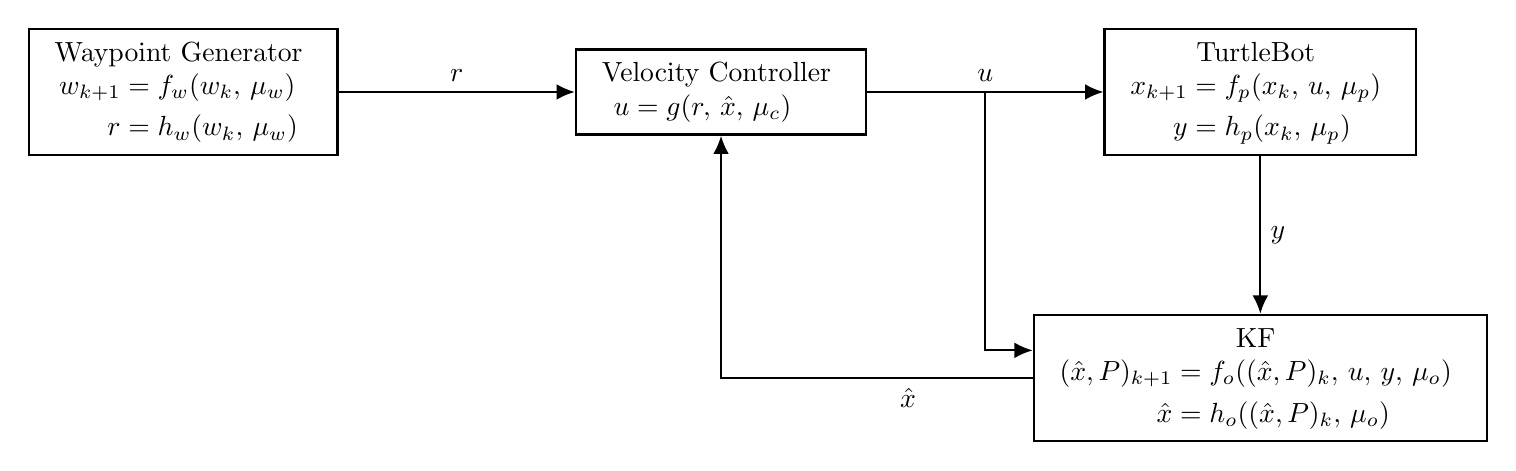
\begin{tikzpicture}[
  block/.style = {draw, thick, minimum height=3em, minimum width=6em, align=center},
  arrow/.style = {thick, -{Latex[width=2mm]}},
  node distance=2.5cm and 2.5cm
]

  % Waypoint Generator
  \node[block] (waypoint) {
    \begin{tabular}{c}
       Waypoint Generator \\
      $\begin{aligned}
      w_{k+1} &= f_w(w_k,\,\mu_w) \\
      r &= h_w(w_k,\,\mu_{w})
       \end{aligned}$
    \end{tabular}
  };

  % Controller (stateless function)
  \node[block, right=3.0cm of waypoint] (controller) {
    \begin{tabular}{c}
            Velocity Controller\\
      $\begin{aligned}
      u &= g(r,\,\hat{x},\,\mu_c)
       \end{aligned}$
    \end{tabular}
  };

  % Plant
  \node[block, right=3.0cm of controller] (plant) {
    \begin{tabular}{c}
      TurtleBot\\
      $\begin{aligned}
      x_{k+1} &= f_p(x_k,\,u,\,\mu_p) \\
      y &= h_p(x_k,\,\mu_{p})
       \end{aligned}$
    \end{tabular}
  };

  % Observer
  \node[block, below=2cm of plant] (observer) {
    \begin{tabular}{c}
      KF\\
    $\begin{aligned}
      (\hat{x}, P)_{k+1} &= f_o((\hat{x}, P)_k,\,u,\,y,\,\mu_o) \\
      \hat{x} &= h_o((\hat{x}, P)_k,\,\mu_{o})
       \end{aligned}$
    \end{tabular}
  };

  % r -> controller
  \draw[arrow] (waypoint.east) -- node[above] {$r$} (controller.west);

  % controller -> plant
  \draw[arrow] (controller.east) -- node[above] {$u$} (plant.west);

  % u branch to observer
  \coordinate (usplit) at ($(controller.east)!0.5!(plant.west)$);
  \coordinate[above=1em of observer.west] (observer_uin);
  \draw[arrow] (usplit) |- (observer_uin);

  % y -> observer
  \draw[arrow] (plant.south) -- node[right] {$y$} (observer.north);

  % observer -> controller (state estimate)
  \draw[arrow] (observer.west) -| node[pos=0.2, below] {$\hat{x}$} (controller.south);

\end{tikzpicture}
\end{document}
